\section{}





\subsection*{Dualer Körper}

Bevor wir mit der Aufgabe selbst beginnen, merken wir zunächst an, dass man anstelle des Oktaeders auch den Würfel benutzen könnte, da es sich um \emph{duale} platonische Körper handelt:
Der zu einem Polyeder $P$ duale Polyeder $P'$ hat als Knotenmenge die Mittelpunkte der Seiten von $P$, und je zwei Mittelpunkte sind genau dann durch eine Kante verbunden, wenn die entsprechenden Seiten aneinander liegen.
\begin{itemize}
  \item
    Der zum Würfel duale Körper ist der Oktaeder:
    \begin{center}
      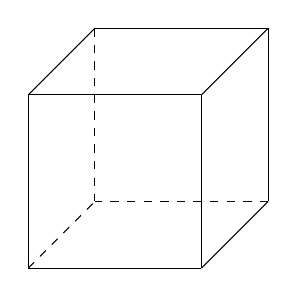
\begin{tikzpicture}[scale=1.1]
        % coordinates for the cube
        \coordinate (fronttopleft)      at  (-1,  1,  1);
        \coordinate (fronttopright)     at  ( 1,  1,  1);
        \coordinate (frontbottomleft)   at  (-1, -1,  1);
        \coordinate (frontbottomright)  at  ( 1, -1,  1);
        \coordinate (backtopleft)       at  (-1,  1, -1);
        \coordinate (backtopright)      at  ( 1,  1, -1);
        \coordinate (backbottomleft)    at  (-1, -1, -1);
        \coordinate (backbottomright)   at  ( 1, -1, -1);
        % drawing the cube
        \draw (fronttopleft)      -- (fronttopright);
        \draw (fronttopleft)      -- (frontbottomleft);
        \draw (fronttopleft)      -- (backtopleft);
        \draw (fronttopright)     -- (frontbottomright);
        \draw (fronttopright)     -- (backtopright);
        \draw (frontbottomleft)   -- (frontbottomright);
        \draw (frontbottomright)  -- (backbottomright);
        \draw (backtopleft)       -- (backtopright);
        \draw (backtopright)      -- (backbottomright);
        \draw[dashed] (backtopleft)     -- (backbottomleft);
        \draw[dashed] (frontbottomleft) -- (backbottomleft);
        \draw[dashed] (backbottomright) -- (backbottomleft);
      \end{tikzpicture}
      \hspace{3em}
      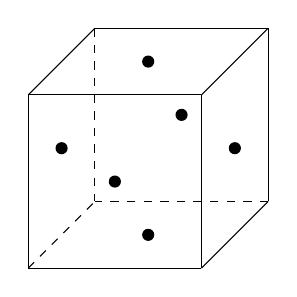
\begin{tikzpicture}[scale=1.1]
        % coordinates for the cube
        \coordinate (fronttopleft)      at  (-1,  1,  1);
        \coordinate (fronttopright)     at  ( 1,  1,  1);
        \coordinate (frontbottomleft)   at  (-1, -1,  1);
        \coordinate (frontbottomright)  at  ( 1, -1,  1);
        \coordinate (backtopleft)       at  (-1,  1, -1);
        \coordinate (backtopright)      at  ( 1,  1, -1);
        \coordinate (backbottomleft)    at  (-1, -1, -1);
        \coordinate (backbottomright)   at  ( 1, -1, -1);
        %coordinates for the octrahedron
        \coordinate (left)    at (-1, 0, 0);
        \coordinate (right)   at ( 1, 0, 0);
        \coordinate (top)     at ( 0, 1, 0);
        \coordinate (bottom)  at ( 0,-1, 0);
        \coordinate (front)   at ( 0, 0, 1);
        \coordinate (back)    at ( 0, 0,-1);
        % drawing the cube
        \draw (fronttopleft)      -- (fronttopright);
        \draw (fronttopleft)      -- (frontbottomleft);
        \draw (fronttopleft)      -- (backtopleft);
        \draw (fronttopright)     -- (frontbottomright);
        \draw (fronttopright)     -- (backtopright);
        \draw (frontbottomleft)   -- (frontbottomright);
        \draw (frontbottomright)  -- (backbottomright);
        \draw (backtopleft)       -- (backtopright);
        \draw (backtopright)      -- (backbottomright);
        \draw[dashed] (backtopleft)     -- (backbottomleft);
        \draw[dashed] (frontbottomleft) -- (backbottomleft);
        \draw[dashed] (backbottomright) -- (backbottomleft);
        % drawing the center of the sides of the cube
        \fill[black]  (left)   circle (0.07);
        \fill[black]  (right)  circle (0.07);
        \fill[black]  (top)    circle (0.07);
        \fill[black]  (bottom) circle (0.07);
        \fill[black]  (front)  circle (0.07);
        \fill[black]  (back)   circle (0.07);
      \end{tikzpicture}
      \hspace{3em}
      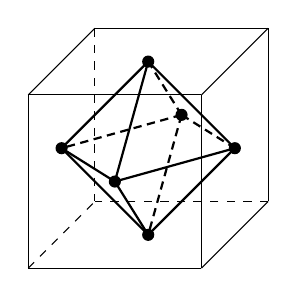
\begin{tikzpicture}[scale=1.1]
        % coordinates for the cube
        \coordinate (fronttopleft)      at  (-1,  1,  1);
        \coordinate (fronttopright)     at  ( 1,  1,  1);
        \coordinate (frontbottomleft)   at  (-1, -1,  1);
        \coordinate (frontbottomright)  at  ( 1, -1,  1);
        \coordinate (backtopleft)       at  (-1,  1, -1);
        \coordinate (backtopright)      at  ( 1,  1, -1);
        \coordinate (backbottomleft)    at  (-1, -1, -1);
        \coordinate (backbottomright)   at  ( 1, -1, -1);
        % coordinates for the octrahedron
        \coordinate (left)    at (-1, 0, 0);
        \coordinate (right)   at ( 1, 0, 0);
        \coordinate (top)     at ( 0, 1, 0);
        \coordinate (bottom)  at ( 0,-1, 0);
        \coordinate (front)   at ( 0, 0, 1);
        \coordinate (back)    at ( 0, 0,-1);
        % drawing the cube
        \draw (fronttopleft)      -- (fronttopright);
        \draw (fronttopleft)      -- (frontbottomleft);
        \draw (fronttopleft)      -- (backtopleft);
        \draw (fronttopright)     -- (frontbottomright);
        \draw (fronttopright)     -- (backtopright);
        \draw (frontbottomleft)   -- (frontbottomright);
        \draw (frontbottomright)  -- (backbottomright);
        \draw (backtopleft)       -- (backtopright);
        \draw (backtopright)      -- (backbottomright);
        \draw[dashed] (backtopleft)     -- (backbottomleft);
        \draw[dashed] (frontbottomleft) -- (backbottomleft);
        \draw[dashed] (backbottomright) -- (backbottomleft);
        % drawing the center of the sides of the cube
        \fill[black]  (left)   circle (0.07);
        \fill[black]  (right)  circle (0.07);
        \fill[black]  (top)    circle (0.07);
        \fill[black]  (bottom) circle (0.07);
        \fill[black]  (front)  circle (0.07);
        \fill[black]  (back)   circle (0.07);
        % drawing the octrahedron
        \draw[thick]  (front)  -- (left);
        \draw[thick]  (front)  -- (right);
        \draw[thick]  (front)  -- (top);
        \draw[thick]  (front)  -- (bottom);
        \draw[thick]  (top)    -- (left);
        \draw[thick]  (top)    -- (right);
        \draw[thick]  (bottom) -- (left);
        \draw[thick]  (bottom) -- (right);
        \draw[thick, densely dashed]  (back) -- (left);
        \draw[thick, densely dashed]  (back) -- (right);
        \draw[thick, densely dashed]  (back) -- (top);
        \draw[thick, densely dashed]  (back) -- (bottom);
      \end{tikzpicture}
    \end{center}
  
  \item
    Der zum Oktaeder duale Körper ist der Würfel:
    \begin{center}
      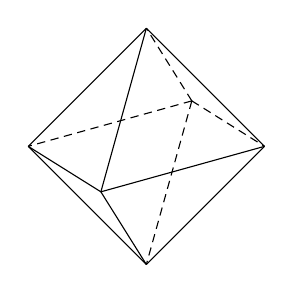
\begin{tikzpicture}[scale=1.5]
        % coordinates for the octrahedron
        \coordinate (left)    at (-1, 0, 0);
        \coordinate (right)   at ( 1, 0, 0);
        \coordinate (top)     at ( 0, 1, 0);
        \coordinate (bottom)  at ( 0,-1, 0);
        \coordinate (front)   at ( 0, 0, 1);
        \coordinate (back)    at ( 0, 0,-1);
        % drawing the octrahedron
        \draw (front)  -- (left);
        \draw (front)  -- (right);
        \draw (front)  -- (top);
        \draw (front)  -- (bottom);
        \draw (top)    -- (left);
        \draw (top)    -- (right);
        \draw (bottom) -- (left);
        \draw (bottom) -- (right);
        \draw[densely dashed] (back) -- (left);
        \draw[densely dashed] (back) -- (right);
        \draw[densely dashed] (back) -- (top);
        \draw[densely dashed] (back) -- (bottom);
      \end{tikzpicture}
      \hspace{3em}
      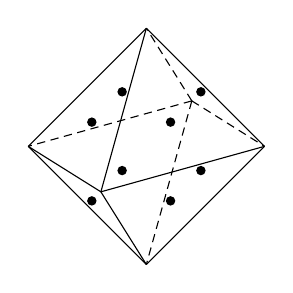
\begin{tikzpicture}[scale=1.5]
        % coordinates for the octrahedron
        \coordinate (left)    at (-1, 0, 0);
        \coordinate (right)   at ( 1, 0, 0);
        \coordinate (top)     at ( 0, 1, 0);
        \coordinate (bottom)  at ( 0,-1, 0);
        \coordinate (front)   at ( 0, 0, 1);
        \coordinate (back)    at ( 0, 0,-1);
        % coordinates for the cube
        \coordinate (fronttopleft)      at  (-1/3,  1/3,  1/3);
        \coordinate (fronttopright)     at  ( 1/3,  1/3,  1/3);
        \coordinate (frontbottomleft)   at  (-1/3, -1/3,  1/3);
        \coordinate (frontbottomright)  at  ( 1/3, -1/3,  1/3);
        \coordinate (backtopleft)       at  (-1/3,  1/3, -1/3);
        \coordinate (backtopright)      at  ( 1/3,  1/3, -1/3);
        \coordinate (backbottomleft)    at  (-1/3, -1/3, -1/3);
        \coordinate (backbottomright)   at  ( 1/3, -1/3, -1/3);
        % drawing the octrahedron
        \draw (front)  -- (left);
        \draw (front)  -- (right);
        \draw (front)  -- (top);
        \draw (front)  -- (bottom);
        \draw (top)    -- (left);
        \draw (top)    -- (right);
        \draw (bottom) -- (left);
        \draw (bottom) -- (right);
        \draw[densely dashed] (back) -- (left);
        \draw[densely dashed] (back) -- (right);
        \draw[densely dashed] (back) -- (top);
        \draw[densely dashed] (back) -- (bottom);
        % drawing the centers of the sides of the octrahedron
        \fill[black]  (fronttopleft)     circle (0.04);
        \fill[black]  (fronttopright)    circle (0.04);
        \fill[black]  (frontbottomleft)  circle (0.04);
        \fill[black]  (frontbottomright) circle (0.04);
        \fill[black]  (backtopleft)      circle (0.04);
        \fill[black]  (backtopright)     circle (0.04);
        \fill[black]  (backbottomleft)   circle (0.04);
        \fill[black]  (backbottomright)  circle (0.04);
      \end{tikzpicture}
      \hspace{3em}
      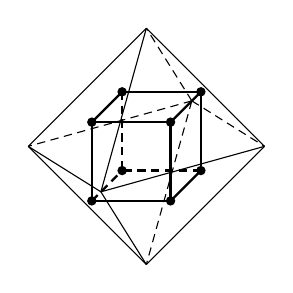
\begin{tikzpicture}[scale=1.5]
        % coordinates for the octrahedron
        \coordinate (left)    at (-1, 0, 0);
        \coordinate (right)   at ( 1, 0, 0);
        \coordinate (top)     at ( 0, 1, 0);
        \coordinate (bottom)  at ( 0,-1, 0);
        \coordinate (front)   at ( 0, 0, 1);
        \coordinate (back)    at ( 0, 0,-1);
        % coordinates for the cube
        \coordinate (fronttopleft)      at  (-1/3,  1/3,  1/3);
        \coordinate (fronttopright)     at  ( 1/3,  1/3,  1/3);
        \coordinate (frontbottomleft)   at  (-1/3, -1/3,  1/3);
        \coordinate (frontbottomright)  at  ( 1/3, -1/3,  1/3);
        \coordinate (backtopleft)       at  (-1/3,  1/3, -1/3);
        \coordinate (backtopright)      at  ( 1/3,  1/3, -1/3);
        \coordinate (backbottomleft)    at  (-1/3, -1/3, -1/3);
        \coordinate (backbottomright)   at  ( 1/3, -1/3, -1/3);
        % drawing the octrahedron
        \draw (front)  -- (left);
        \draw (front)  -- (right);
        \draw (front)  -- (top);
        \draw (front)  -- (bottom);
        \draw (top)    -- (left);
        \draw (top)    -- (right);
        \draw (bottom) -- (left);
        \draw (bottom) -- (right);
        \draw[densely dashed] (back) -- (left);
        \draw[densely dashed] (back) -- (right);
        \draw[densely dashed] (back) -- (top);
        \draw[densely dashed] (back) -- (bottom);
        % drawing the centers of the sides of the octrahedron
        \fill[black]  (fronttopleft)     circle (0.04);
        \fill[black]  (fronttopright)    circle (0.04);
        \fill[black]  (frontbottomleft)  circle (0.04);
        \fill[black]  (frontbottomright) circle (0.04);
        \fill[black]  (backtopleft)      circle (0.04);
        \fill[black]  (backtopright)     circle (0.04);
        \fill[black]  (backbottomleft)   circle (0.04);
        \fill[black]  (backbottomright)  circle (0.04);
        % drawing the cube
        \draw[thick]  (fronttopleft)      -- (fronttopright);
        \draw[thick]  (fronttopleft)      -- (frontbottomleft);
        \draw[thick]  (fronttopleft)      -- (backtopleft);
        \draw[thick]  (fronttopright)     -- (frontbottomright);
        \draw[thick]  (fronttopright)     -- (backtopright);
        \draw[thick]  (frontbottomleft)   -- (frontbottomright);
        \draw[thick]  (frontbottomright)  -- (backbottomright);
        \draw[thick]  (backtopleft)       -- (backtopright);
        \draw[thick]  (backtopright)      -- (backbottomright);
        \draw[thick, densely dashed]  (backtopleft)     -- (backbottomleft);
        \draw[thick, densely dashed]  (frontbottomleft) -- (backbottomleft);
        \draw[thick, densely dashed]  (backbottomright) -- (backbottomleft);
      \end{tikzpicture}
    \end{center}
\end{itemize}

Da Oktaeder und Würfel dual zueinander sind, haben beide Körper die gleiche Isometriegruppe.
Wir werden uns im Folgenden aber den Oktaeder nutzen (wie in der Aufgabenstellung).





\subsection*{Elemente von $\Okt$}

Wir geben mehrere Möglichkeiten an, die Anzahl der Elemente von $\Okt$ zu bestimmen:
\begin{itemize}
  \item 
    Im Oktaeder gibt es drei Vierecke:
    \begin{center}
      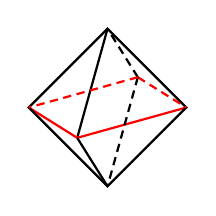
\begin{tikzpicture}[scale = 1]
        \coordinate (right)   at ( 1, 0, 0);
        \coordinate (left)    at (-1, 0, 0);
        \coordinate (top)     at ( 0, 1, 0);
        \coordinate (bottom)  at ( 0,-1, 0);
        \coordinate (front)   at ( 0, 0, 1);
        \coordinate (back)    at ( 0, 0,-1);
        \draw[thick]        (front) -- (top);
        \draw[thick,red]    (front) -- (right);
        \draw[thick]        (front) -- (bottom);
        \draw[thick,red]    (front) -- (left);
        \draw[thick]        (top) -- (right) -- (bottom) -- (left) -- cycle;
        \draw[densely dashed,thick]     (back) -- (top);
        \draw[densely dashed,thick,red] (back) -- (right);
        \draw[densely dashed,thick]     (back) -- (bottom);
        \draw[densely dashed,thick,red] (back) -- (left);
      \end{tikzpicture}
      \hspace{3em}
      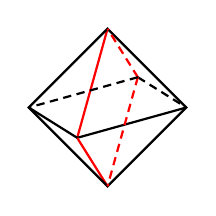
\begin{tikzpicture}[scale = 1]
        \coordinate (right)   at ( 1, 0, 0);
        \coordinate (left)    at (-1, 0, 0);
        \coordinate (top)     at ( 0, 1, 0);
        \coordinate (bottom)  at ( 0,-1, 0);
        \coordinate (front)   at ( 0, 0, 1);
        \coordinate (back)    at ( 0, 0,-1);
        \draw[thick,red]    (front) -- (top);
        \draw[thick]        (front) -- (right);
        \draw[thick,red]    (front) -- (bottom);
        \draw[thick]        (front) -- (left);
        \draw[thick]        (top) -- (right) -- (bottom) -- (left) -- cycle;
        \draw[densely dashed,thick,red] (back) -- (top);
        \draw[densely dashed,thick]     (back) -- (right);
        \draw[densely dashed,thick,red] (back) -- (bottom);
        \draw[densely dashed,thick]     (back) -- (left);
      \end{tikzpicture}
      \hspace{3em}
      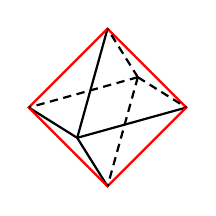
\begin{tikzpicture}[scale = 1]
        \coordinate (right)   at ( 1, 0, 0);
        \coordinate (left)    at (-1, 0, 0);
        \coordinate (top)     at ( 0, 1, 0);
        \coordinate (bottom)  at ( 0,-1, 0);
        \coordinate (front)   at ( 0, 0, 1);
        \coordinate (back)    at ( 0, 0,-1);
        \draw[thick]        (front) -- (top);
        \draw[thick]        (front) -- (right);
        \draw[thick]        (front) -- (bottom);
        \draw[thick]        (front) -- (left);
        \draw[thick,red]    (top) -- (right) -- (bottom) -- (left) -- cycle;
        \draw[densely dashed,thick] (back) -- (top);
        \draw[densely dashed,thick] (back) -- (right);
        \draw[densely dashed,thick] (back) -- (bottom);
        \draw[densely dashed,thick] (back) -- (left);
      \end{tikzpicture}
    \end{center}
    Wir bezeichnen mit $Q$ das erste der Quadrate.

    Jede Isometrie des Oktaeders muss diese drei Vierecke permutieren, d.h.\ $\Okt$ wirkt auf der dreielementigen Menge der Vierecke.
    Diese Wirkung ist transitv, da sich $Q$ durch passende Drehungen zu den beiden anderen Quadraten umwandeln lässt.
    Bezeichnet $H \coloneqq \Okt_Q$ den Stabilisator des ausgewählten Quadrats $Q$, so gilt also $|{\Okt}|/|H| = 3$.
    Es genügt daher im Folgenden, die Kardinalität der Untergruppe $H$ zu bestimmen.

    Es gibt zwei Eckpunkte, $P_1$ und $P_2$, die sich nicht in dem ausgewählten Quadrat befinden:
    \begin{center}
        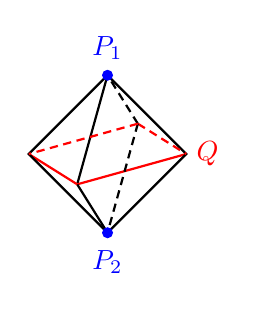
\begin{tikzpicture}[scale = 1]
        \coordinate (right)   at ( 1, 0, 0);
        \coordinate (left)    at (-1, 0, 0);
        \coordinate (top)     at ( 0, 1, 0);
        \coordinate (bottom)  at ( 0,-1, 0);
        \coordinate (front)   at ( 0, 0, 1);
        \coordinate (back)    at ( 0, 0,-1);
        \draw[thick]        (front) -- (top);
        \draw[thick,red]    (front) -- (right) node[anchor=west] {$Q$};
        \draw[thick]        (front) -- (bottom);
        \draw[thick,red]    (front) -- (left);
        \draw[thick]        (top) -- (right) -- (bottom) -- (left) -- cycle;
        \draw[densely dashed,thick]     (back) -- (top);
        \draw[densely dashed,thick,red] (back) -- (right);
        \draw[densely dashed,thick]     (back) -- (bottom);
        \draw[densely dashed,thick,red] (back) -- (left);
        \fill[blue] (top)     circle (0.07) node[above = 2] {$P_1$};
        \fill[blue] (bottom)  circle (0.07) node[below = 3] {$P_2$};
      \end{tikzpicture}
    \end{center}
    Jede Isometrie des Oktaeders, welche das Quadrat $Q$ fixiert, muss diese beiden Eckpunkte permutieren, d.h.\ die Gruppe $H$ wirkt auf $\{P_1, P_2\}$.
    Diese Wirkung ist transitiv, denn $H$ enthält die Spiegelung an der $Q$-Ebene, und diese Spiegelung bildet $P_1$ auf $P_2$ ab.
    Für den Stabilisator $K \coloneqq H_{P_1}$ gilt somit, dass $|H|/|K| = 2$.
    Es genügt daher, die Kardinalität der Untergruppe $K$ zu bestimmen.
    
    Die Isometrien des Oktaeders, welche die Eckpunkte $P_1$ und $P_2$ fixieren, entsprechen genau den Isometrien des Quadrats $Q$.
    Es gilt also $K \cong D_4$, und somit $|K| = |D_4| = 8$.
    Somit gilt
    \[
        |{\Okt}|
      = 3 \cdot 2 \cdot |K|
      = 3 \cdot 2 \cdot 8
      = 48.
    \]
    
  \item
    Wir können den Oktaeder so in den Raum $\Real^3$ einbetten, dass die Eckpunkte des Oktaeders genau die Punkte $\pm e_i$ sind:
    \begin{center}
        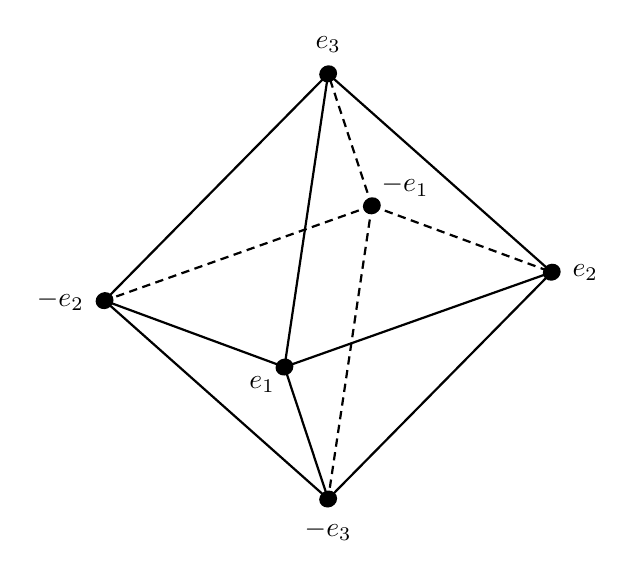
\begin{tikzpicture}[scale = 2.7, rotate around y=10]
        \coordinate (right)   at ( 1, 0, 0);
        \coordinate (left)    at (-1, 0, 0);
        \coordinate (top)     at ( 0, 1, 0);
        \coordinate (bottom)  at ( 0,-1, 0);
        \coordinate (front)   at ( 0, 0, 1);
        \coordinate (back)    at ( 0, 0,-1);
        \draw[thick]        (front) -- (top);
        \draw[thick]        (front) -- (right);
        \draw[thick]        (front) -- (bottom);
        \draw[thick]        (front) -- (left);
        \draw[thick]        (top) -- (right) -- (bottom) -- (left) -- cycle;
        \draw[densely dashed,thick]     (back) -- (top);
        \draw[densely dashed,thick]     (back) -- (right);
        \draw[densely dashed,thick]     (back) -- (bottom);
        \draw[densely dashed,thick]     (back) -- (left);
        \fill[black] (top)    circle (0.04) node[above = 4] {$e_3$};
        \fill[black] (bottom) circle (0.04) node[below = 4] {$-e_3$};
        \fill[black] (right)  circle (0.04) node[right = 4] {$e_2$};
        \fill[black] (left)   circle (0.04) node[left = 4] {$-e_2$};
        \fill[black] (front)   circle (0.04) node[anchor = north east] {$e_1$};
        \fill[black] (back)   circle (0.04) node[anchor = south west] {$-e_1$};
      \end{tikzpicture}
    \end{center}
    Jede Isometrie des Oktaeders bildet gegenüberliegende Eckpunkte auf gegenüberliegende Eckpunkte ab;
    deshalb liefert jede Isometrie $w \in \Okt$ des Oktaeders eine Vorzeichenpermutation $\pi_w \in \signper{3}$:
    Falls $w$ den Eckpunkt $e_i$ auf den Eckpunkt $\varepsilon e_j$ mit $\varepsilon = \pm 1$ abbildet, so gilt $\pi_w(i) = \varepsilon j$.
    Hierdurch ergibt sich ein Gruppenhomomorphismus $\varphi \colon \Okt \to \signper{3}$, $w \mapsto \pi_w$.
    Jede Isometrie des Oktaeders ist durch die Wirkung auf den Eckpunkten bereits eindeutig bestimmt, weshalb $\varphi$ injektiv ist.
    
    Die Spiegelung an der $e_1$-$e_2$-Ebene wird auf die Vorzeichenpermutation $\pi \in \signper{3}$ mit $\pi(3) = -3$ und $\pi(\pm i) = \pm i$ für $i = 1, 2$ abgebildet, d.h.\ auf den Vorzeichenwechsel von $3$.
    \begin{center}
        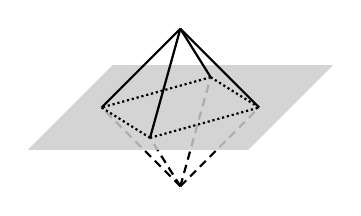
\begin{tikzpicture}[scale = 1]
        \coordinate (right)   at ( 1, 0, 0);
        \coordinate (left)    at (-1, 0, 0);
        \coordinate (top)     at ( 0, 1, 0);
        \coordinate (bottom)  at ( 0,-1, 0);
        \coordinate (front)   at ( 0, 0, 1);
        \coordinate (back)    at ( 0, 0,-1);
        \draw[densely dashed,thick]                (bottom) -- (front);
        \draw[densely dashed,thick]                (bottom) -- (left);
        \draw[densely dashed,thick]                (bottom) -- (right);
        \draw[densely dashed,thick] (bottom) -- (back);
        \fill[gray!40!white, opacity=0.85] (1.4, 0, 1.4) -- (1.4, 0, -1.4) -- (-1.4, 0, -1.4) -- (-1.4, 0, 1.4) -- cycle;
        \draw[densely dotted,thick]                (front) -- (left);
        \draw[densely dotted,thick]                (front) -- (right);
        \draw[densely dotted,thick] (back) -- (left);
        \draw[densely dotted,thick] (back) -- (right);
        \draw[thick]                (top) -- (front);
        \draw[thick]                (top) -- (left);
        \draw[thick]                (top) -- (right);
        \draw[thick] (top) -- (back);
      \end{tikzpicture}
    \end{center}
    Analog ergibt sich, dass auch die anderen beiden Vorzeichenwechsel im Bild von $\varphi$ liegen.
    Betrachtet man die Spiegelung an der $(e_1\!+\!e_2)$-$e_3$-Ebene, so wird diese auf die Transposition $(1 \; 2) \in S_3 \subgroup \signper{3}$ abgebildet.    
    \begin{center}
        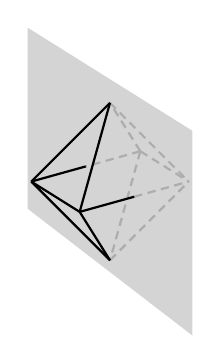
\begin{tikzpicture}[scale = 1]
        \coordinate (right)       at ( 1,   0,  0);
        \coordinate (left)        at (-1,   0,  0);
        \coordinate (top)         at ( 0,   1,  0);
        \coordinate (bottom)      at ( 0,  -1,  0);
        \coordinate (front)       at ( 0,   0,  1);
        \coordinate (frontright)  at ( 0.5, 0,  0.5);
        \coordinate (backleft)    at (-0.5, 0, -0.5);
        \coordinate (back)        at ( 0,   0, -1);
        \draw[densely dashed,thick] (back) -- (top);
        \draw[densely dashed,thick] (back) -- (bottom);
        \draw[densely dashed,thick] (back) -- (backleft);
        \draw[densely dashed,thick] (back) -- (right);
        \draw[densely dashed,thick] (bottom) -- (right);
        \draw[densely dashed,thick] (frontright) -- (right);
        \draw[densely dashed,thick] (top) -- (right);
        \fill[gray!40!white, opacity=0.85] (1.7,1.3,1.7) -- (-1.7,1.3,-1.7) -- (-1.7,-1.,-1.7) -- (1.7,-1.3,1.7) -- cycle;
        \draw[thick]  (front) -- (top);
        \draw[thick]  (front) -- (bottom);
        \draw[thick]  (front) -- (left);
        \draw[thick]  (front) -- (frontright);
        \draw[thick]  (top) -- (left);
        \draw[thick]  (bottom) -- (left);
        \draw[thick]  (left) -- (backleft);
%         \draw[densely dotted] (top) -- (backleft) -- (bottom) -- (frontright) -- cycle;
      \end{tikzpicture}
    \end{center}
    Analog ergibt sich, dass auch alle anderen Transpositionen aus $S_3$ im Bild von $\varphi$ liegen.
    Da $\signper{3}$ von den Vorzeichenwechseln und Transpositionen erzeugt wird, ergibt sich damit insgesamt, dass $\varphi$ surjektiv ist.
    
    Der Gruppenhomomorphismus $\varphi$ ist also bereits ein Isomorphismus.
    Somit gilt $\Okt \cong\signper{3}$, und insbesondere $|\Okt| = |\signper{3}| = 2^3 \cdot 3! = 8 \cdot 6 = 48$.
    
  \item
    Es sei $P$ ein beliebiger Eckpunkt des Oktaeders.
    Durch die Isometrien des Oktaeders lässt sich der Eckpunkt $P$ auf jeden der Eckpunkte abbilden;
    für den Bildpunkt $P'$ von $P$ gibt es also $6$ Möglichkeiten.
    
    Es sei $Q$ ein zu $P$ benachbarter Eckpunkt.
    Durch die Isometrien des Oktaeders wird $Q$ auf einen zu $P'$ benachbarten Eckpunkt abgebildet;
    durch eventuelles Nachschalten mit Rotationen um die $P'$-Achse lässt sich dabei jeder zu $P'$ benachbarten Eckpunkte erreichen.
    Für den Bildpunkt $Q'$ von $Q$ gibt es also $4$ Möglichkeiten.
    
    Es sei $R$ ein zu $P$ und $Q$ benachbarter Eckpunkt.
    Die Isometrien des Quaders bilden $R$ auf einen zu $P'$ und $Q'$ benachbarten Eckpunkt ab;
    durch eventuelles Nachschalten mit der Spiegelung an der $P'$-$Q'$-Ebene können dabei beide mögliche Eckpunkte erreicht werden.
    Für den Bildpunkt $R'$ von $R$ gibt es also $2$ Möglichkeiten.
    
    Durch die Wirkung auf den drei benachbarten Eckpunkten $P$, $Q$ und $R$ sind die Isometrien des Oktaeders bereits eindeutig bestimmt.
    Also gilt $|\Okt| = 6 \cdot 4 \cdot 2 = 48$.
\end{itemize}

Alternativ lassen sich die $48$ Isometrien des Oktraheders auch explizit auflisten.
Dies wird hier aus den folgenden Gründen nicht getan:
\begin{itemize}
  \item
    Ohne eines der obigen Argumentationen ist nicht klar, ob man alle Isometrien gefunden hat.
  \item
    Der Autor hat keine Lust, $48$ weitere Bilder zu zeichnen.
  \item
    Wir benötigen im Folgenden keine explizite Beschreibung aller Isometrien.
\end{itemize}
Wer dennoch eine vollständige Liste aller Isometrien haben möchte, kann online eine Liste aller Isometrien des Würfels finden\footnote{Siehe \url{www.pentoma.de/symmetrien-von-figuren-aus-wuerfeln}.} und nutzten, dass der Oktaeder dual zum Würfel ist.





\subsection*{Gruppenhomomorphismen $h \colon \Okt \to \Integer/2$ und $t \colon \Integer/2 \to \Okt$}

Wir können den Oktaeder so in den Raum $\Real^3$ einbetten, so dass die Achsen des Oktaeders auf den Koordinatenachsen liegen.
\begin{center}
    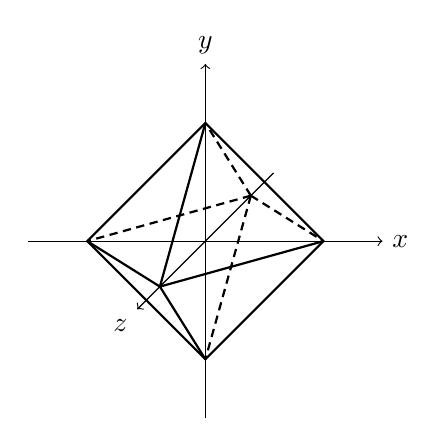
\begin{tikzpicture}[scale = 1.5]
    \coordinate (right)   at ( 1, 0, 0);
    \coordinate (left)    at (-1, 0, 0);
    \coordinate (top)     at ( 0, 1, 0);
    \coordinate (bottom)  at ( 0,-1, 0);
    \coordinate (front)   at ( 0, 0, 1);
    \coordinate (back)    at ( 0, 0,-1);
    \draw[thick]        (front) -- (top);
    \draw[thick]        (front) -- (right);
    \draw[thick]        (front) -- (bottom);
    \draw[thick]        (front) -- (left);
    \draw[thick]        (top) -- (right) -- (bottom) -- (left) -- cycle;
    \draw[densely dashed,thick]     (back) -- (top);
    \draw[densely dashed,thick]     (back) -- (right);
    \draw[densely dashed,thick]     (back) -- (bottom);
    \draw[densely dashed,thick]     (back) -- (left);
    \draw[->] (-1.5, 0, 0) -- (1.5, 0, 0) node[anchor=west] {$x$};
    \draw[->] (0, -1.5, 0) -- (0, 1.5, 0) node[anchor=south] {$y$};
    \draw[->] (0, 0, -1.5) -- (0, 0, 1.5) node[anchor=north east] {$z$};
  \end{tikzpicture}
\end{center}
Damit können die Isometrien des Oktaeders als Isometrien des umgebenden Raums $\Real^3$ aufgefasst werden, und somit als orthogonale Transformationen von $\Real^3$.
Mithilfe der Determinante ergibt sich dann, wie für die Diedergruppen, ein Gruppenhomomorphismus
\[
          h
  \colon  \Okt
  \to     \Integer/2,
  \quad   w
  \mapsto \begin{cases}
            0 & \text{falls $w$ eine Rotation ist}, \\
            1 & \text{falls $w$ eine Spiegelung oder Drehspiegelung ist}.
          \end{cases}
\]
Jede Spiegelung $w \in \Okt$ liefert dann, wie bei den Diedergruppen, einen Gruppenhomomorphismus
\[
          t
  \colon  \Integer/2
  \to     \Okt,
  \quad   \class{n}
  \mapsto w^n
\]
mit $g \circ t = \id_{\Integer/2}$.
Der Kern $\Okt^+ \coloneqq \ker g \subgroup \Okt$ besteht genau aus der Untergruppe der Rotationen.
Es gilt
\[
    \frac{|\Okt|}{|\Okt^+|}
  = |\Integer/2|
  = 2
\]
und somit $|\Okt^+| = |\Okt|/2 = 48/2 = 24$.





\subsection*{Gruppenisomorphismus $\Okt^+ \to S^4$}

Der Oktaeder besteht $4$ Paaren von gegenüberliegenden Seiten.
Wir nummerieren diese Paare mit $1$, $2$, $3$, $4$.
Da jede Isometrie des Oktaeders diese Paare permutiert, erhalten wir einen Gruppenhomomorphismus $k \colon \Okt^+ \to S_4$.
Wir zeigen, dass $k$ bereits ein Isomorphismus ist.
Da $|\Okt^+| = 24 = |S_4|$ gilt, genügt es zu zeigen, dass $k$ surjektiv ist.
Hierfür genügt es zu zeigen, dass $\im k$ alle Transpositionen enthält, da $S_4$ von diesen erzeugt wird.

Hierfür betrachte man die Rotation (um $180^\circ$) um die Gerade, die durch die Mittelpunkte zweier gegenüberliegender Kanten geht.
\begin{center}
    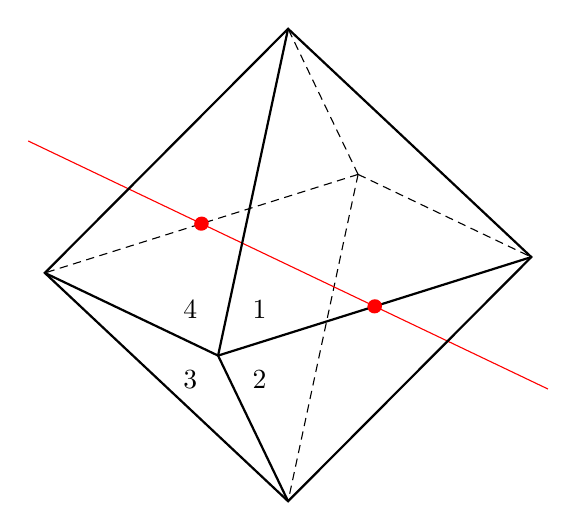
\begin{tikzpicture}[scale = 3, rotate around y=5]
    % coordinates for the octrahedron
    \coordinate (right)       at ( 1,   0,  0);
    \coordinate (left)        at (-1,   0,  0);
    \coordinate (top)         at ( 0,   1,  0);
    \coordinate (bottom)      at ( 0,  -1,  0);
    \coordinate (front)       at ( 0,   0,  1);
    \coordinate (back)        at ( 0,   0, -1);
    \coordinate (frontright)  at ( 0.5, 0,  0.5);
    \coordinate (backleft)    at (-0.5, 0, -0.5);
    % coordinates for the cube
    \draw[thin, densely dashed]     (back) -- (top);
    \draw[thin, densely dashed]     (back) -- (right);
    \draw[thin, densely dashed]     (back) -- (bottom);
    \draw[thin, densely dashed]     (back) -- (left);
    \draw[red] (1.5, 0, 1.5) -- (-1.5, 0, -1.5);
    \draw[thick]  (front) -- (top);
    \draw[thick]  (front) -- (right);
    \draw[thick]  (front) -- (bottom);
    \draw[thick]  (front) -- (left);
    \draw[thick]  (top) -- (right) -- (bottom) -- (left) -- cycle;
    \fill[red]  (frontright)  circle (0.03);
    \fill[red]  (backleft)    circle (0.03);
    \draw (front) node[right=15pt,  above=10pt] {$1$};
    \draw (front) node[right=15pt,  below=2pt]  {$2$};
    \draw (front) node[left=10pt,   below=2pt]  {$3$};
    \draw (front) node[left=10pt,   above=10pt] {$4$};
  \end{tikzpicture}
\end{center}
In dem obigen Beispiel vertauscht die Rotation die beiden Seiten $1$ und $2$, und bildet die Seiten $3$ und $4$ jeweils auf die gegenüberliegende Seite ab.
Von $k$ wird diese Rotation also auf die Transposition $(1 \; 2)$ abgebildet.
Ingesamt gibt es $6$ solche Rotationen, welche wegen der Injektivität von $k$ auf die $6$ Transpositionen in $S_4$ abgebildet werden.

Insgesamt zeigt dies die Surjektivität von $k$, und somit dass $k$ ein Isomorphismus ist.




